\documentclass[12pt]{article}

\usepackage[a4paper, margin=1in]{geometry}
\usepackage{fancyhdr}
\usepackage{titling}
\usepackage{babel}[latvian]
\usepackage{graphicx}
\usepackage{float}
\usepackage{dirtytalk}
\usepackage{gensymb}
\usepackage[utf8]{inputenc}
\usepackage[T1]{fontenc} 
\usepackage{amsmath}

\newlength\tindent
\setlength{\tindent}{\parindent}
\setlength{\parindent}{0pt}
\renewcommand{\indent}{\hspace*{\tindent}}

\fancypagestyle{plain}{
  \fancyhf{}
  \fancyhead[R]{ Andrejs Cvečkovskis \\ ac24005 \\ Kurss \say{Zinātniskā programmēšana fiziķiem}}
  \renewcommand{\headrulewidth}{0pt}
}

\title{\vspace{-1cm}\centering Laboratorijas darbs \\[1ex] \large \say{Siltumvadīšana} \vspace{-6em}}
\author{}
\date{}  
\begin{document}
\maketitle

\section*{Uzsildīta objekta atdzišana}

\begin{enumerate}
  \item Attēls siltumvadīšanas vienādojuma atrisinājumam pie dažādām
        parametra~$\Delta t$ vērtībām un analītiskais atrisinājums.
\begin{center}
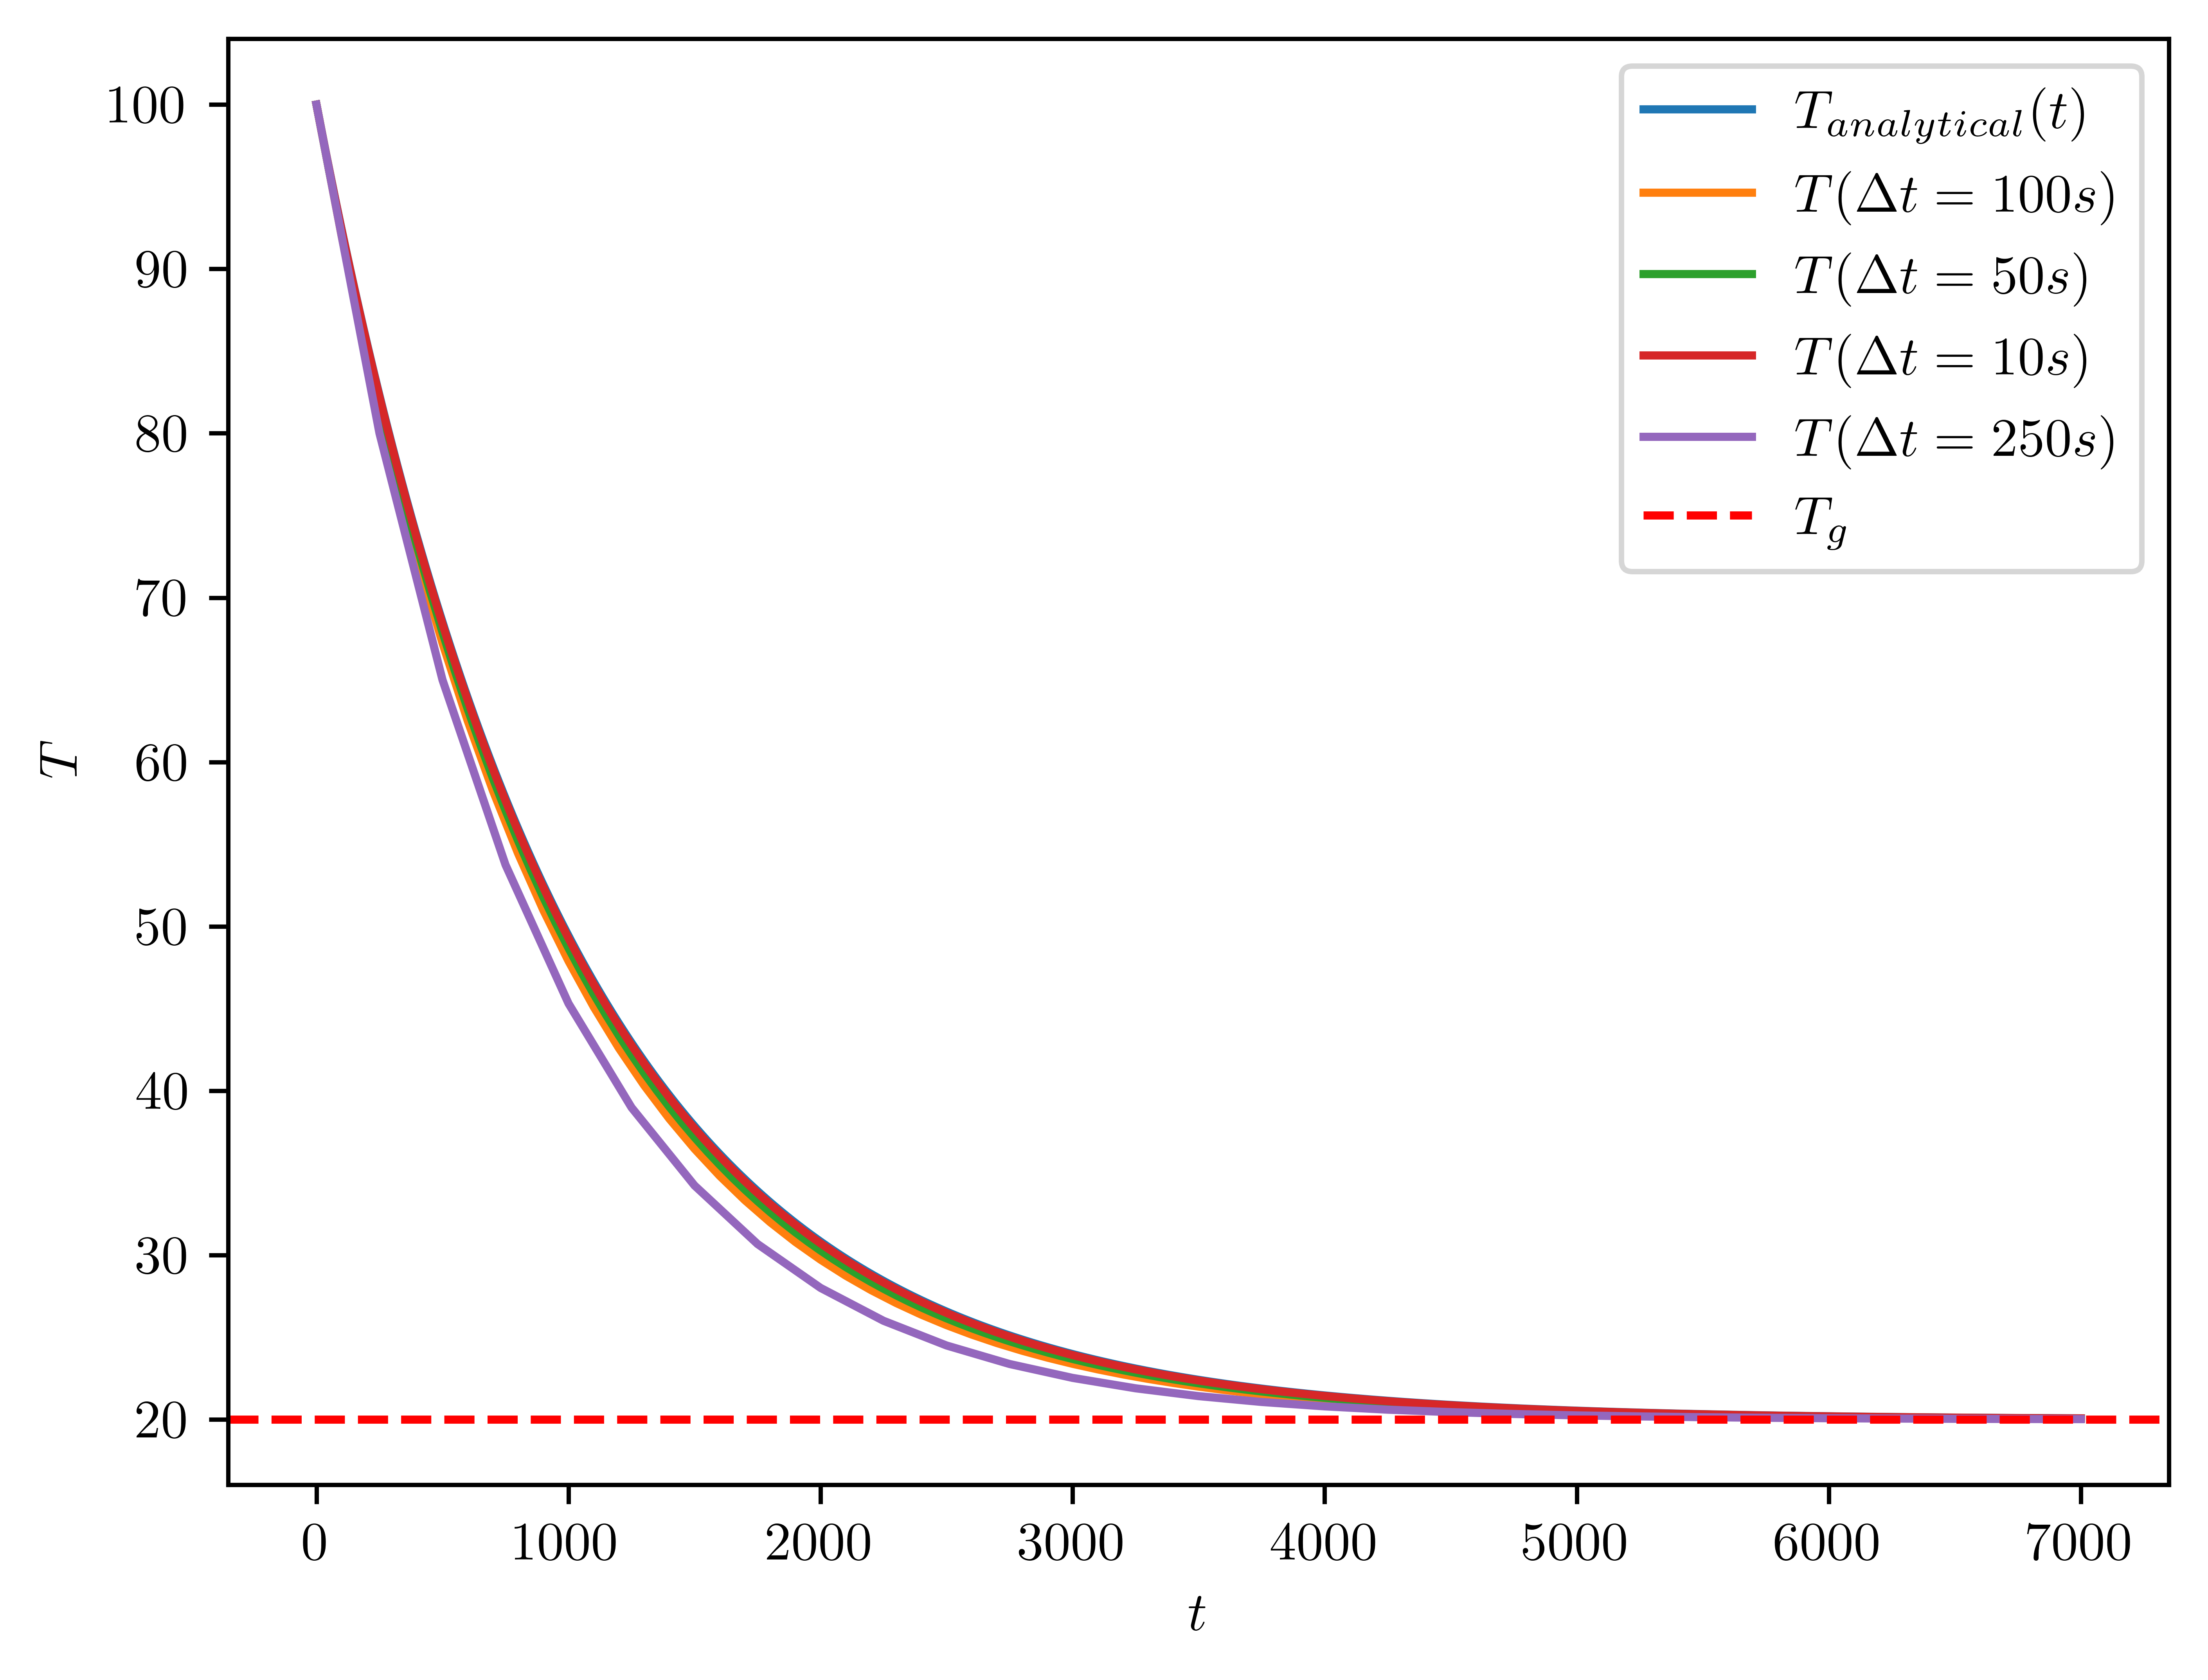
\includegraphics[]{1.1.png}
\end{center}
        
  \item Attēls siltumvadīšanas vienādojuma atrisinājumam,
        kurā novērojamas skaitliskas nestabilitātes.

\begin{center}
    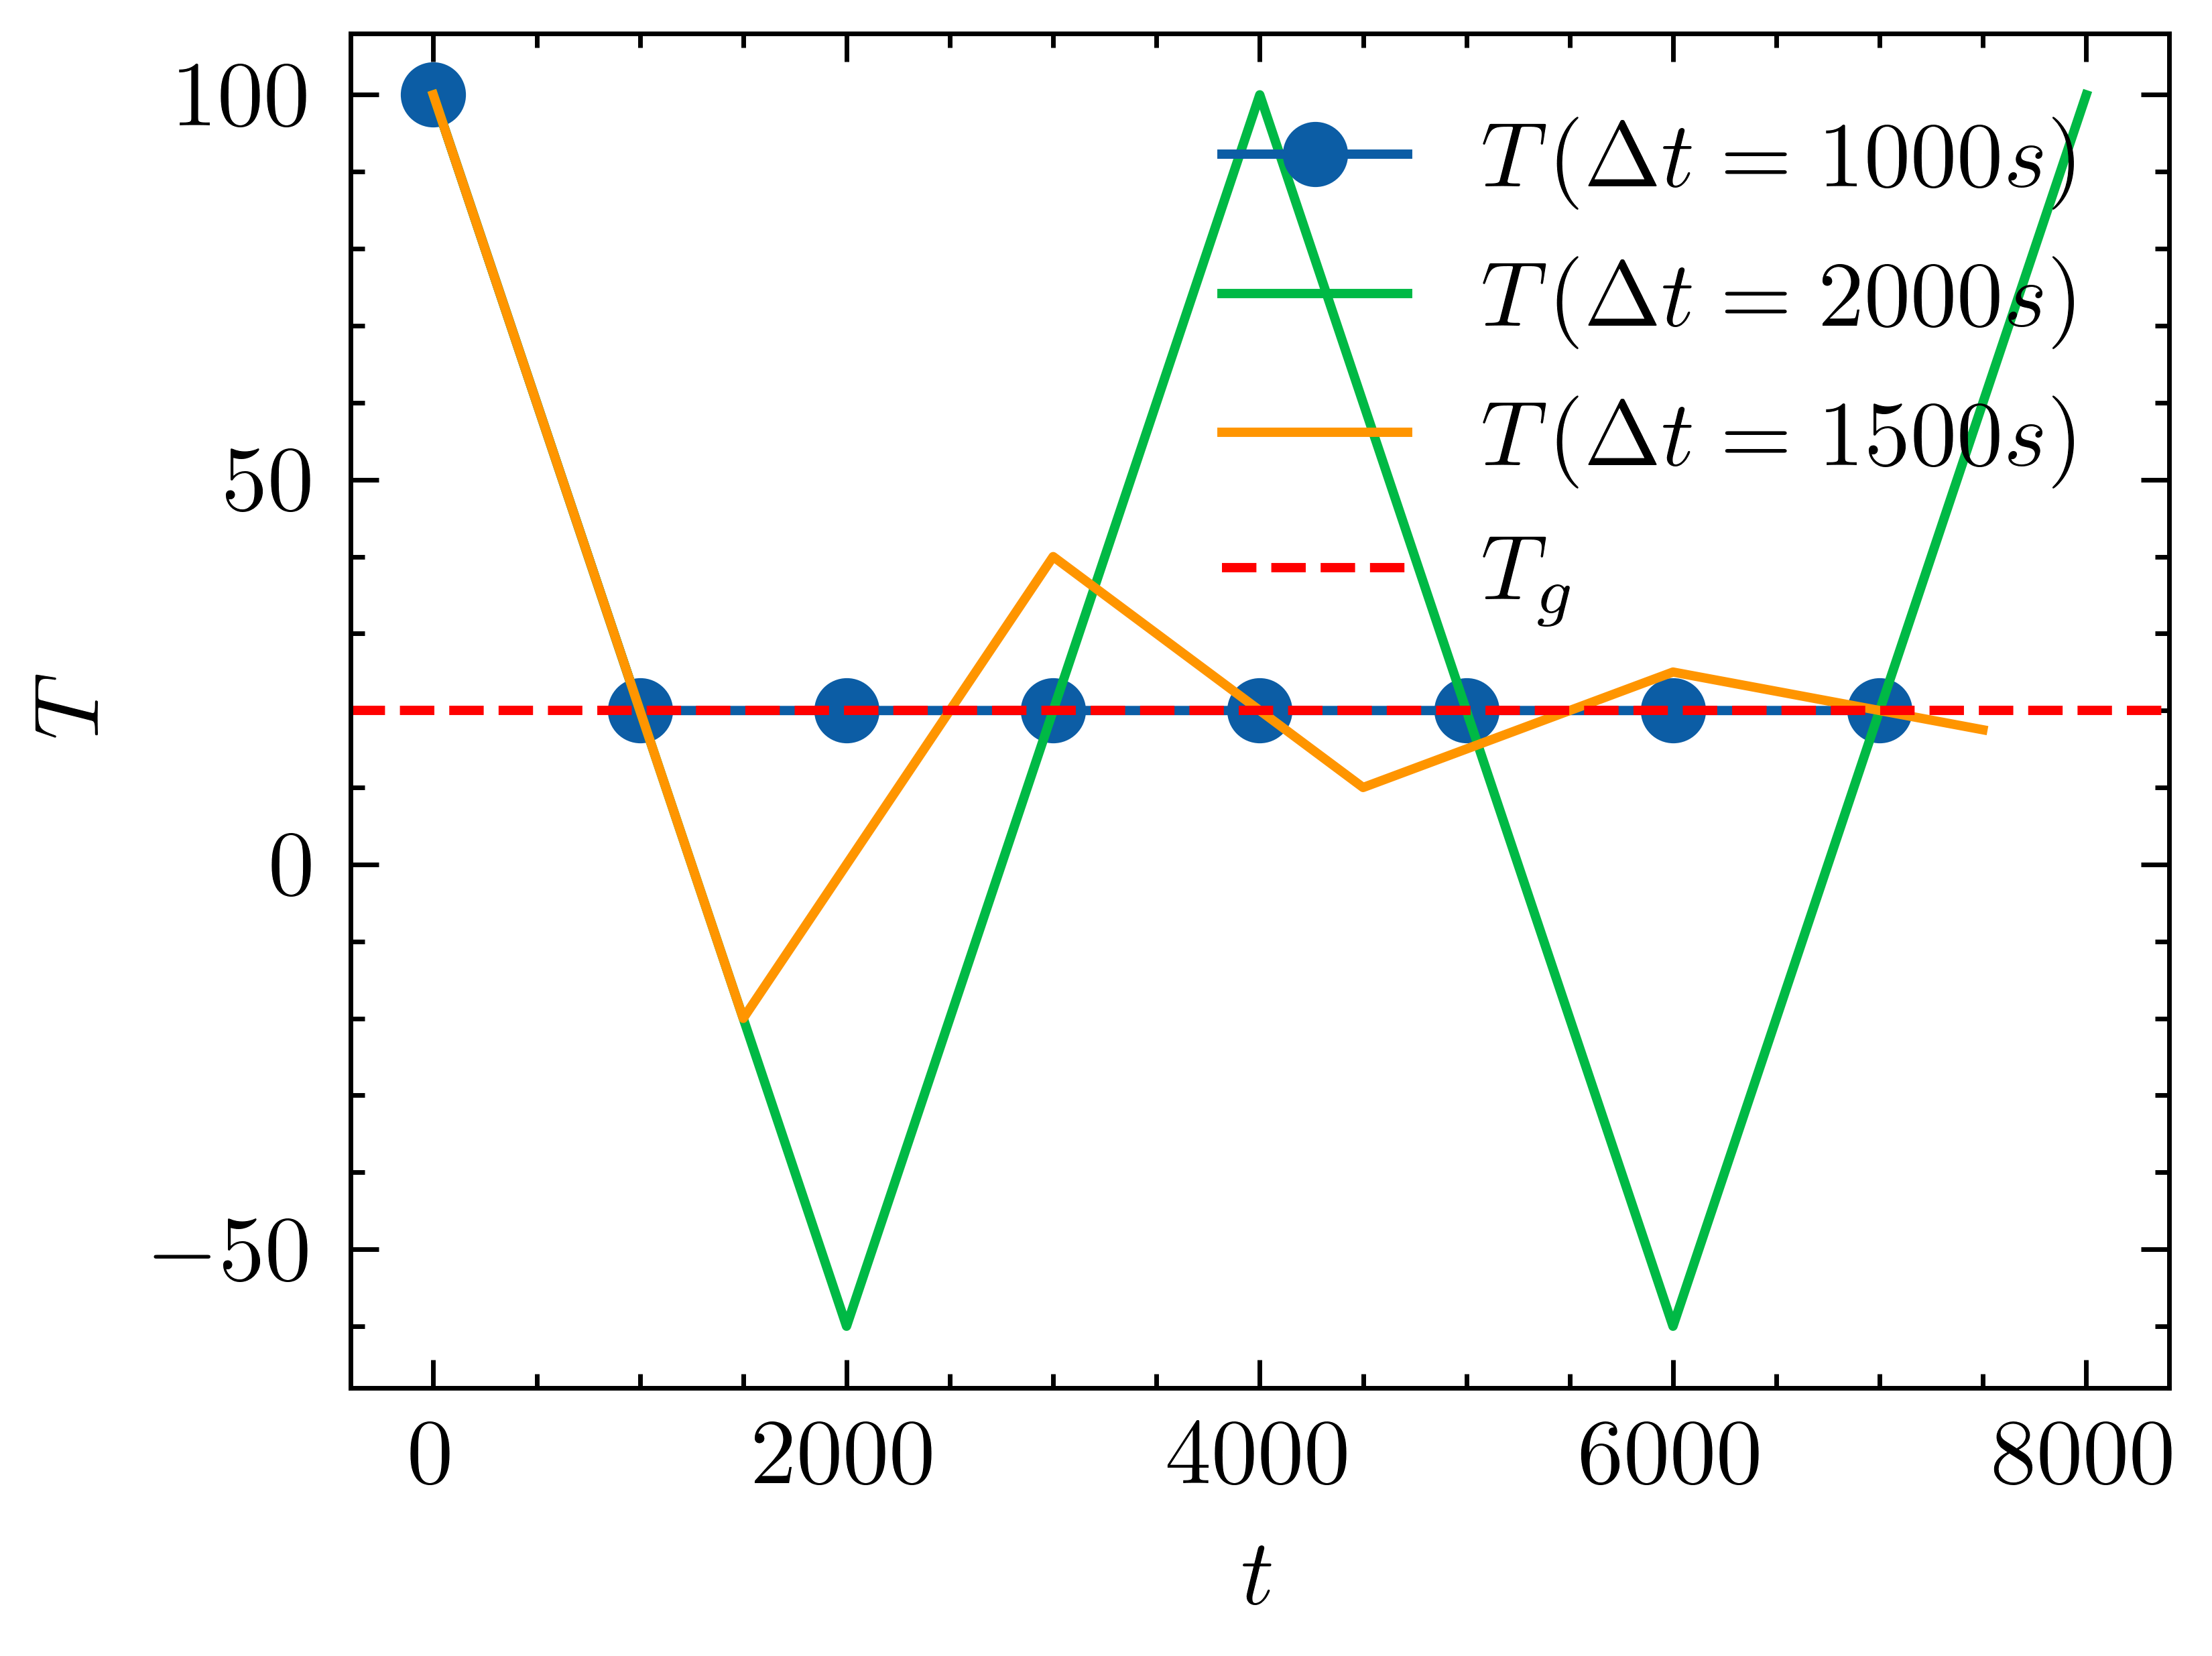
\includegraphics[]{1.2.png}
\end{center}
    
  \item Attēls siltumvadīšanas vienādojuma atrisinājumam ar
        \texttt{solve\_ivp} un analītiskais atrisinājums.

\begin{center}
    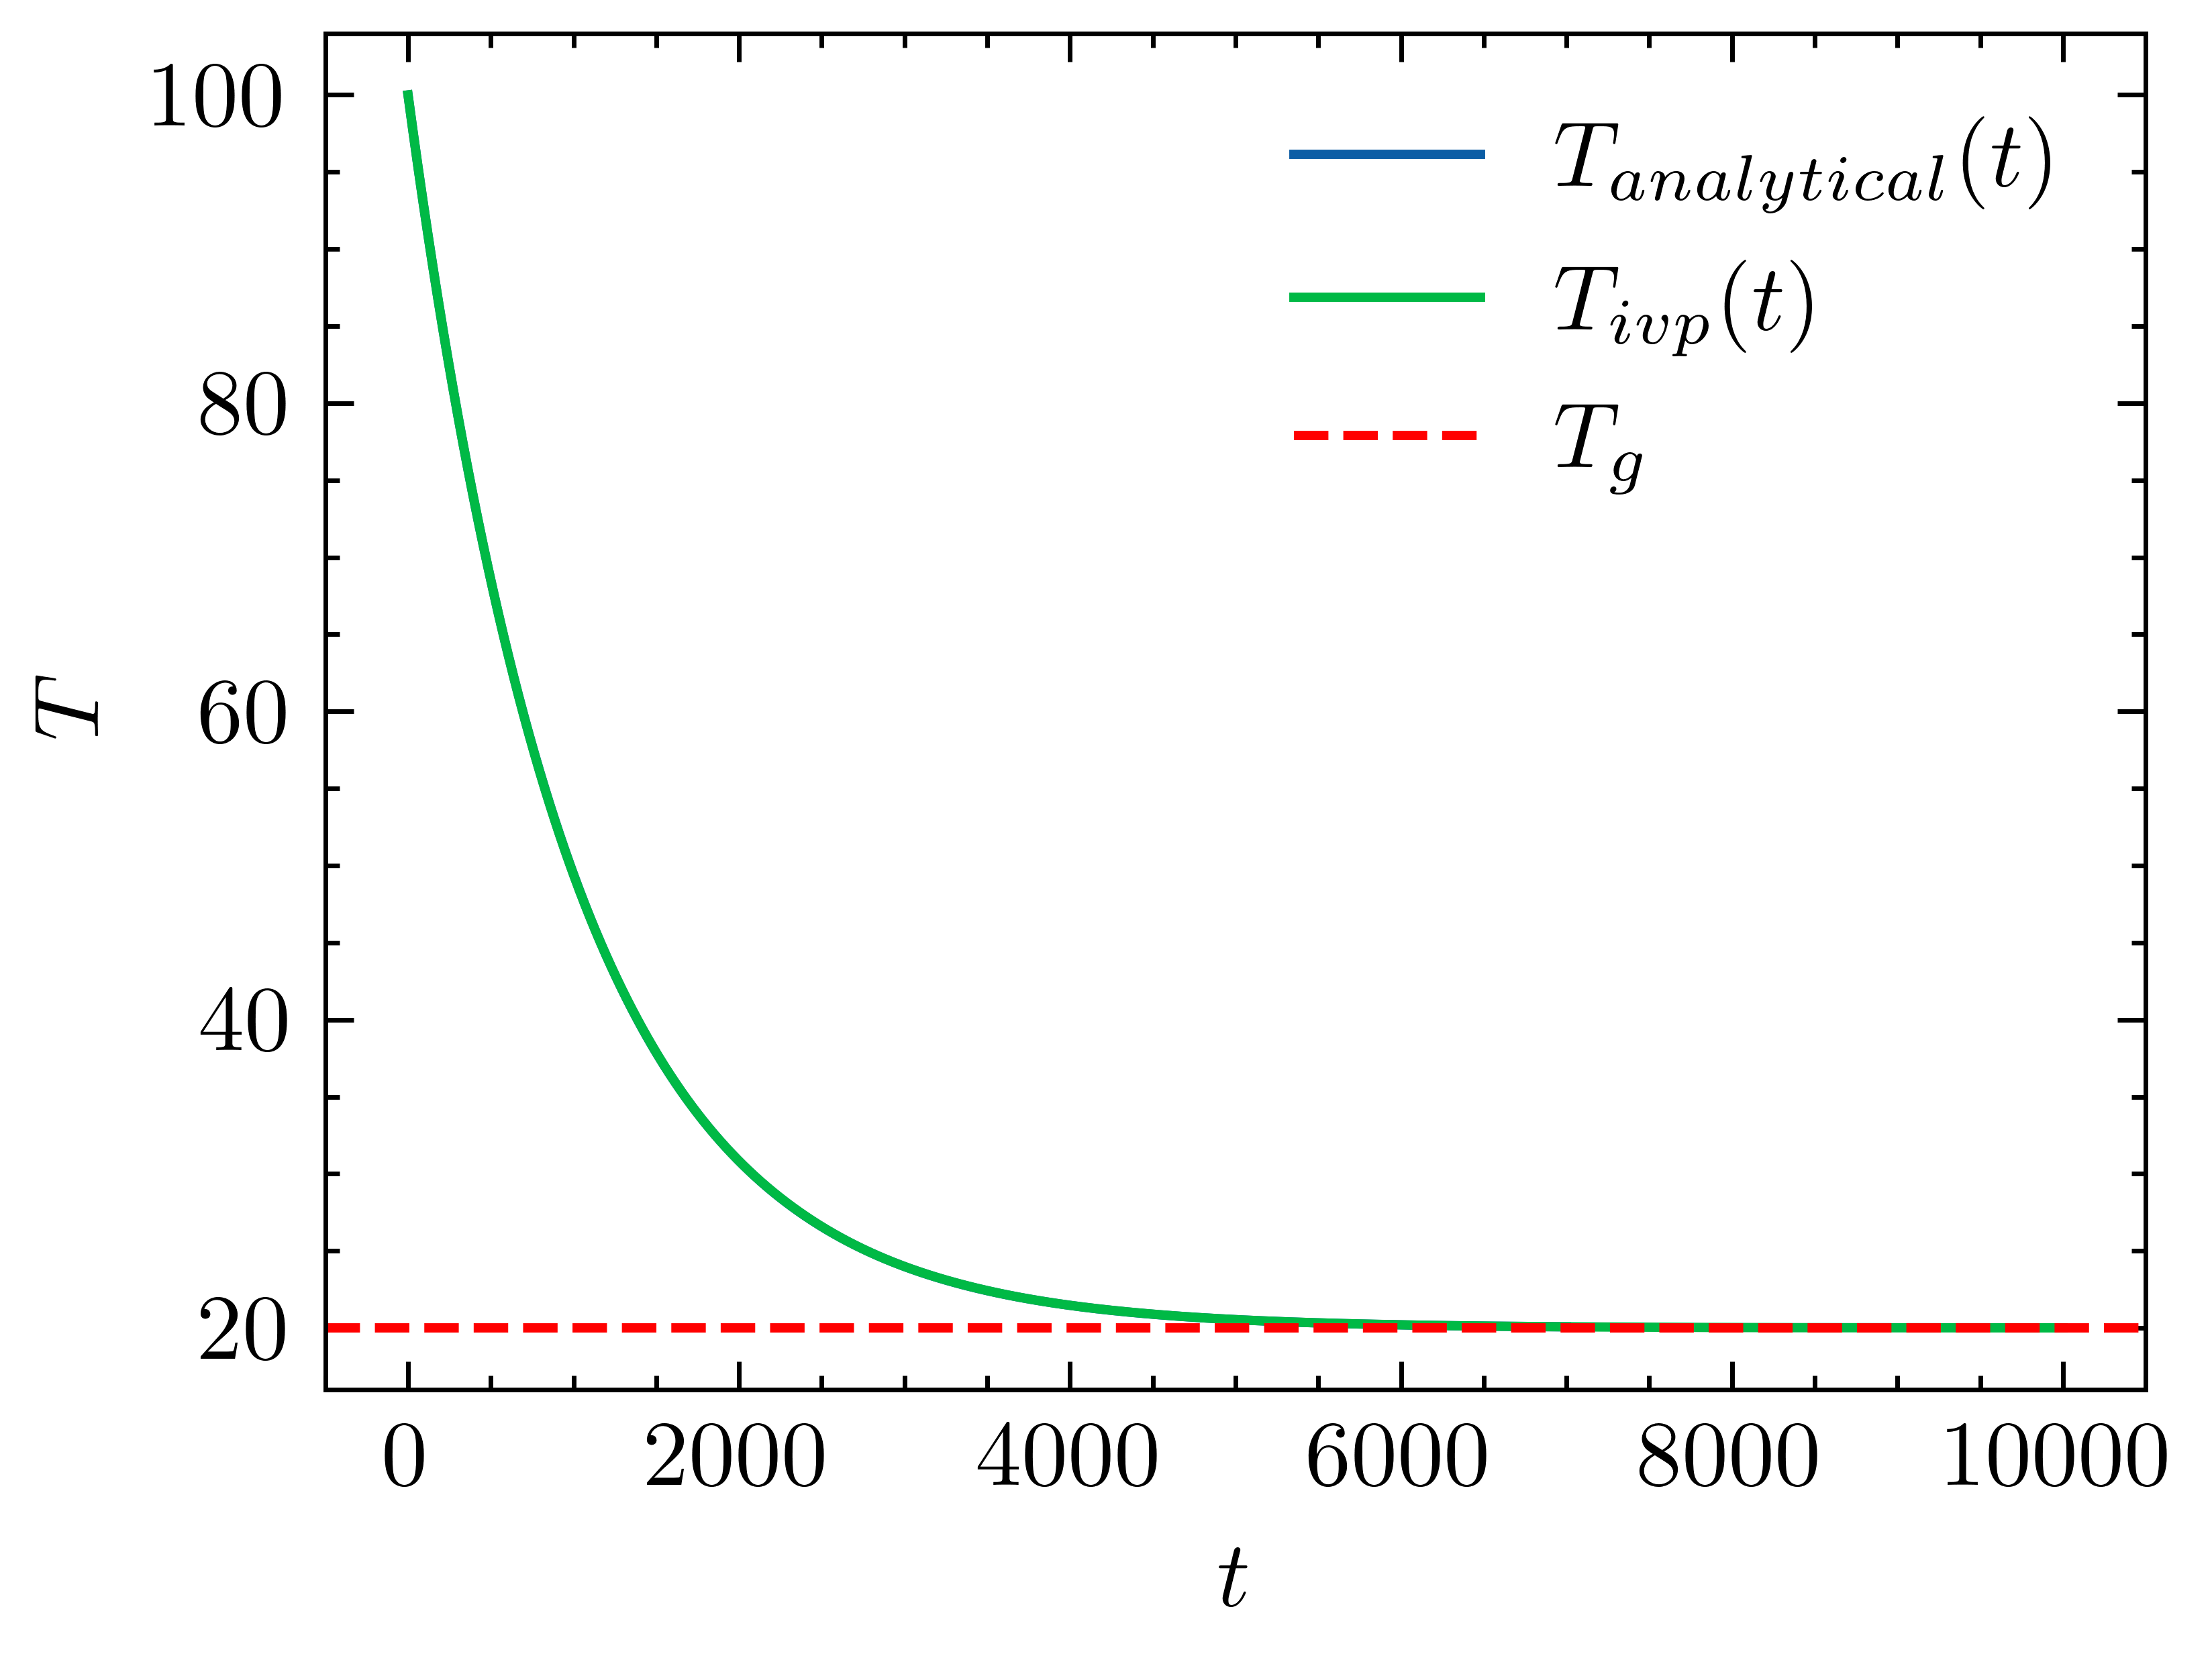
\includegraphics[]{1.3.png}
\end{center}
        
  \item \textbf{PAMATOJUMS:} Izmantotais kods.

\begin{verbatim}
# initial conditions
y0 = [100, 20, 0.001]
T_0 = 100
T_g = 20
coefficient = 1/1000
# solve ivp solution # 3rd sort of point of the protocol
 
def dTdt(t, T, T_g=T_g, k=coefficient):
    return -k*(T - T_g)

# solve
sol = solve_ivp(dTdt, [0, 10000], [T_0], t_eval=np.linspace(0, 10000, 100000))

# plot
fig, ax = plt.subplots()
ax.plot(sol.t, sol.y[0], label=r'$T(t)$')
ax.set_xlabel(r'$t$')
ax.set_ylabel(r'$T$')
ax.axhline(y=20, color='r', linestyle='--', label=r'$T_g$')
ax.legend()
plt.show()

# eulers method # 1st and 2nd point of the protocol
 
dt = 1000
dt1 = 750
dt2 = 500
dt3 = 250
dt4 = 100
dt5 = 50
dt6 = 10
dt7 = 2000
dt8 = 1500
t = np.arange(0, 7000+dt, dt)
t1 = np.arange(0, 7000+dt1, dt1)
t2 = np.arange(0, 7000+dt2, dt2)
t3 = np.arange(0, 7000+dt3, dt3)
t4 = np.arange(0, 7000+dt4, dt4)
t5 = np.arange(0, 7000+dt5, dt5)
t6 = np.arange(0, 7000+dt6, dt6)
t7 = np.arange(0, 7000+dt7, dt7)
t8 = np.arange(0, 7000+dt8, dt8)
T_0 = 100

T_dt2 = np.zeros(len(t2))
T_dt2[0] = T_0

T_dt1 = np.zeros(len(t1))
T_dt1[0] = T_0

T_dt = np.zeros(len(t))
T_dt[0] = T_0

T_dt3 = np.zeros(len(t3))
T_dt3[0] = T_0

T_dt4 = np.zeros(len(t4))
T_dt4[0] = T_0

T_dt5 = np.zeros(len(t5))
T_dt5[0] = T_0

T_dt6 = np.zeros(len(t6))
T_dt6[0] = T_0

T_7d7 = np.zeros(len(t7))
T_7d7[0] = T_0

T_8d8 = np.zeros(len(t8))
T_8d8[0] = T_0

for j in range(0, len(t)-1):
    T_dt[j+1] = T_dt[j] + dt*dTdt(t[j], T_dt[j])

for i in range(0, len(t2)-1):
    T_dt2[i+1] = T_dt2[i] + dt2*dTdt(t2[i], T_dt2[i])

for k in range(0, len(t1)-1):
    T_dt1[k+1] = T_dt1[k] + dt1*dTdt(t1[k], T_dt1[k])

for l in range(0, len(t3)-1):
    T_dt3[l+1] = T_dt3[l] + dt3*dTdt(t3[l], T_dt3[l])

for m in range(0, len(t4)-1):
    T_dt4[m+1] = T_dt4[m] + dt4*dTdt(t4[m], T_dt4[m])

for n in range(0, len(t5)-1):
    T_dt5[n+1] = T_dt5[n] + dt5*dTdt(t5[n], T_dt5[n])

for o in range(0, len(t6)-1):
    T_dt6[o+1] = T_dt6[o] + dt6*dTdt(t6[o], T_dt6[o])

for p in range(0, len(t7)-1):
    T_7d7[p+1] = T_7d7[p] + dt7*dTdt(t7[p], T_7d7[p])

for q in range(0, len(t8)-1):
    T_8d8[q+1] = T_8d8[q] + dt8*dTdt(t8[q], T_8d8[q])

t_ana = np.linspace(0, 7000, 100000)
T_anal = (T_0 - T_g) * np.exp(-coefficient * t_ana) + T_g

fig, ax = plt.subplots()
# ax.plot(t_ana, T_anal, label=r'$T_{analytical}(t)$')
# ax.plot(t4, T_dt4, label=r'$T(\Delta{t=100}s)$')
# ax.plot(t5, T_dt5, label=r'$T(\Delta{t=50}s)$')
# ax.plot(t6, T_dt6, label=r'$T(\Delta{t=10}s)$')
ax.plot(t, T_dt, label=r'$T(\Delta{t=1000}s)$', marker = 'o')
# ax.plot(t3, T_dt3, label=r'$T(\Delta{t=250}s)$')
# ax.plot(t2, T_dt2, label=r'$T(\Delta{t=500}s)$')
# ax.plot(t1, T_dt1, label=r'$T(\Delta{t=750}s)$')
ax.plot(t7, T_7d7, label=r'$T(\Delta{t=2000}s)$')
ax.plot(t8, T_8d8, label=r'$T(\Delta{t=1500}s)$',)
ax.set_xlabel(r'$t$')
ax.set_ylabel(r'$T$')
ax.axhline(y=20, color='r', linestyle='--', label=r'$T_g$')
ax.legend()
plt.savefig(os.path.join(path, '1.2.png'), dpi=1000, bbox_inches='tight')
plt.show()
# analytical solution - shit, 
currently ### to be fixed # 3rd point of the protocol # not shit anymore

t_ana = np.linspace(0, 7000, 10000)
T_anal = (T_0 - T_g) * np.exp(-coefficient * t_ana) + T_g

fig, ax = plt.subplots()
ax.plot(t_ana, T_anal, label=r'$T_{analytical}(t)$')
# ax.plot(t2, T_dt2, label=r'$T(t)_{broken}$') # he just like me :(
ax.plot(sol.t, sol.y[0], label=r'$T_{ivp}(t)$')
ax.set_xlabel(r'$t$')
ax.set_ylabel(r'$T$')
ax.axhline(y=20, color='r', linestyle='--', label=r'$T_g$')
ax.legend()
plt.savefig(os.path.join(path, '1.3.png'), dpi=1000, bbox_inches='tight')
plt.show()
\end{verbatim}
  
\end{enumerate}

\newpage

\section*{Siltumvadīšanas vienādojums}

\begin{enumerate}
  \item Izmantotās parametru vērtības un krūzītes izmēri.
  \begin{verbatim}
rho = 1000.0          # kg/m^3, density of water
cp = 4186.0           # J/(kg·K), specific heat capacity of water
k = 0.5918            # W/(m·K), thermal conductivity of water
  \end{verbatim}
  \item Atrisināt siltumvadīšanas vienādojumu stienī, kur sākuma temperatūra ir $100^\circ C$, bet temperatūra uz stieņa galiem ir $20^\circ C$. \\ Attēls problēmas atrisinājumam.
\begin{center}
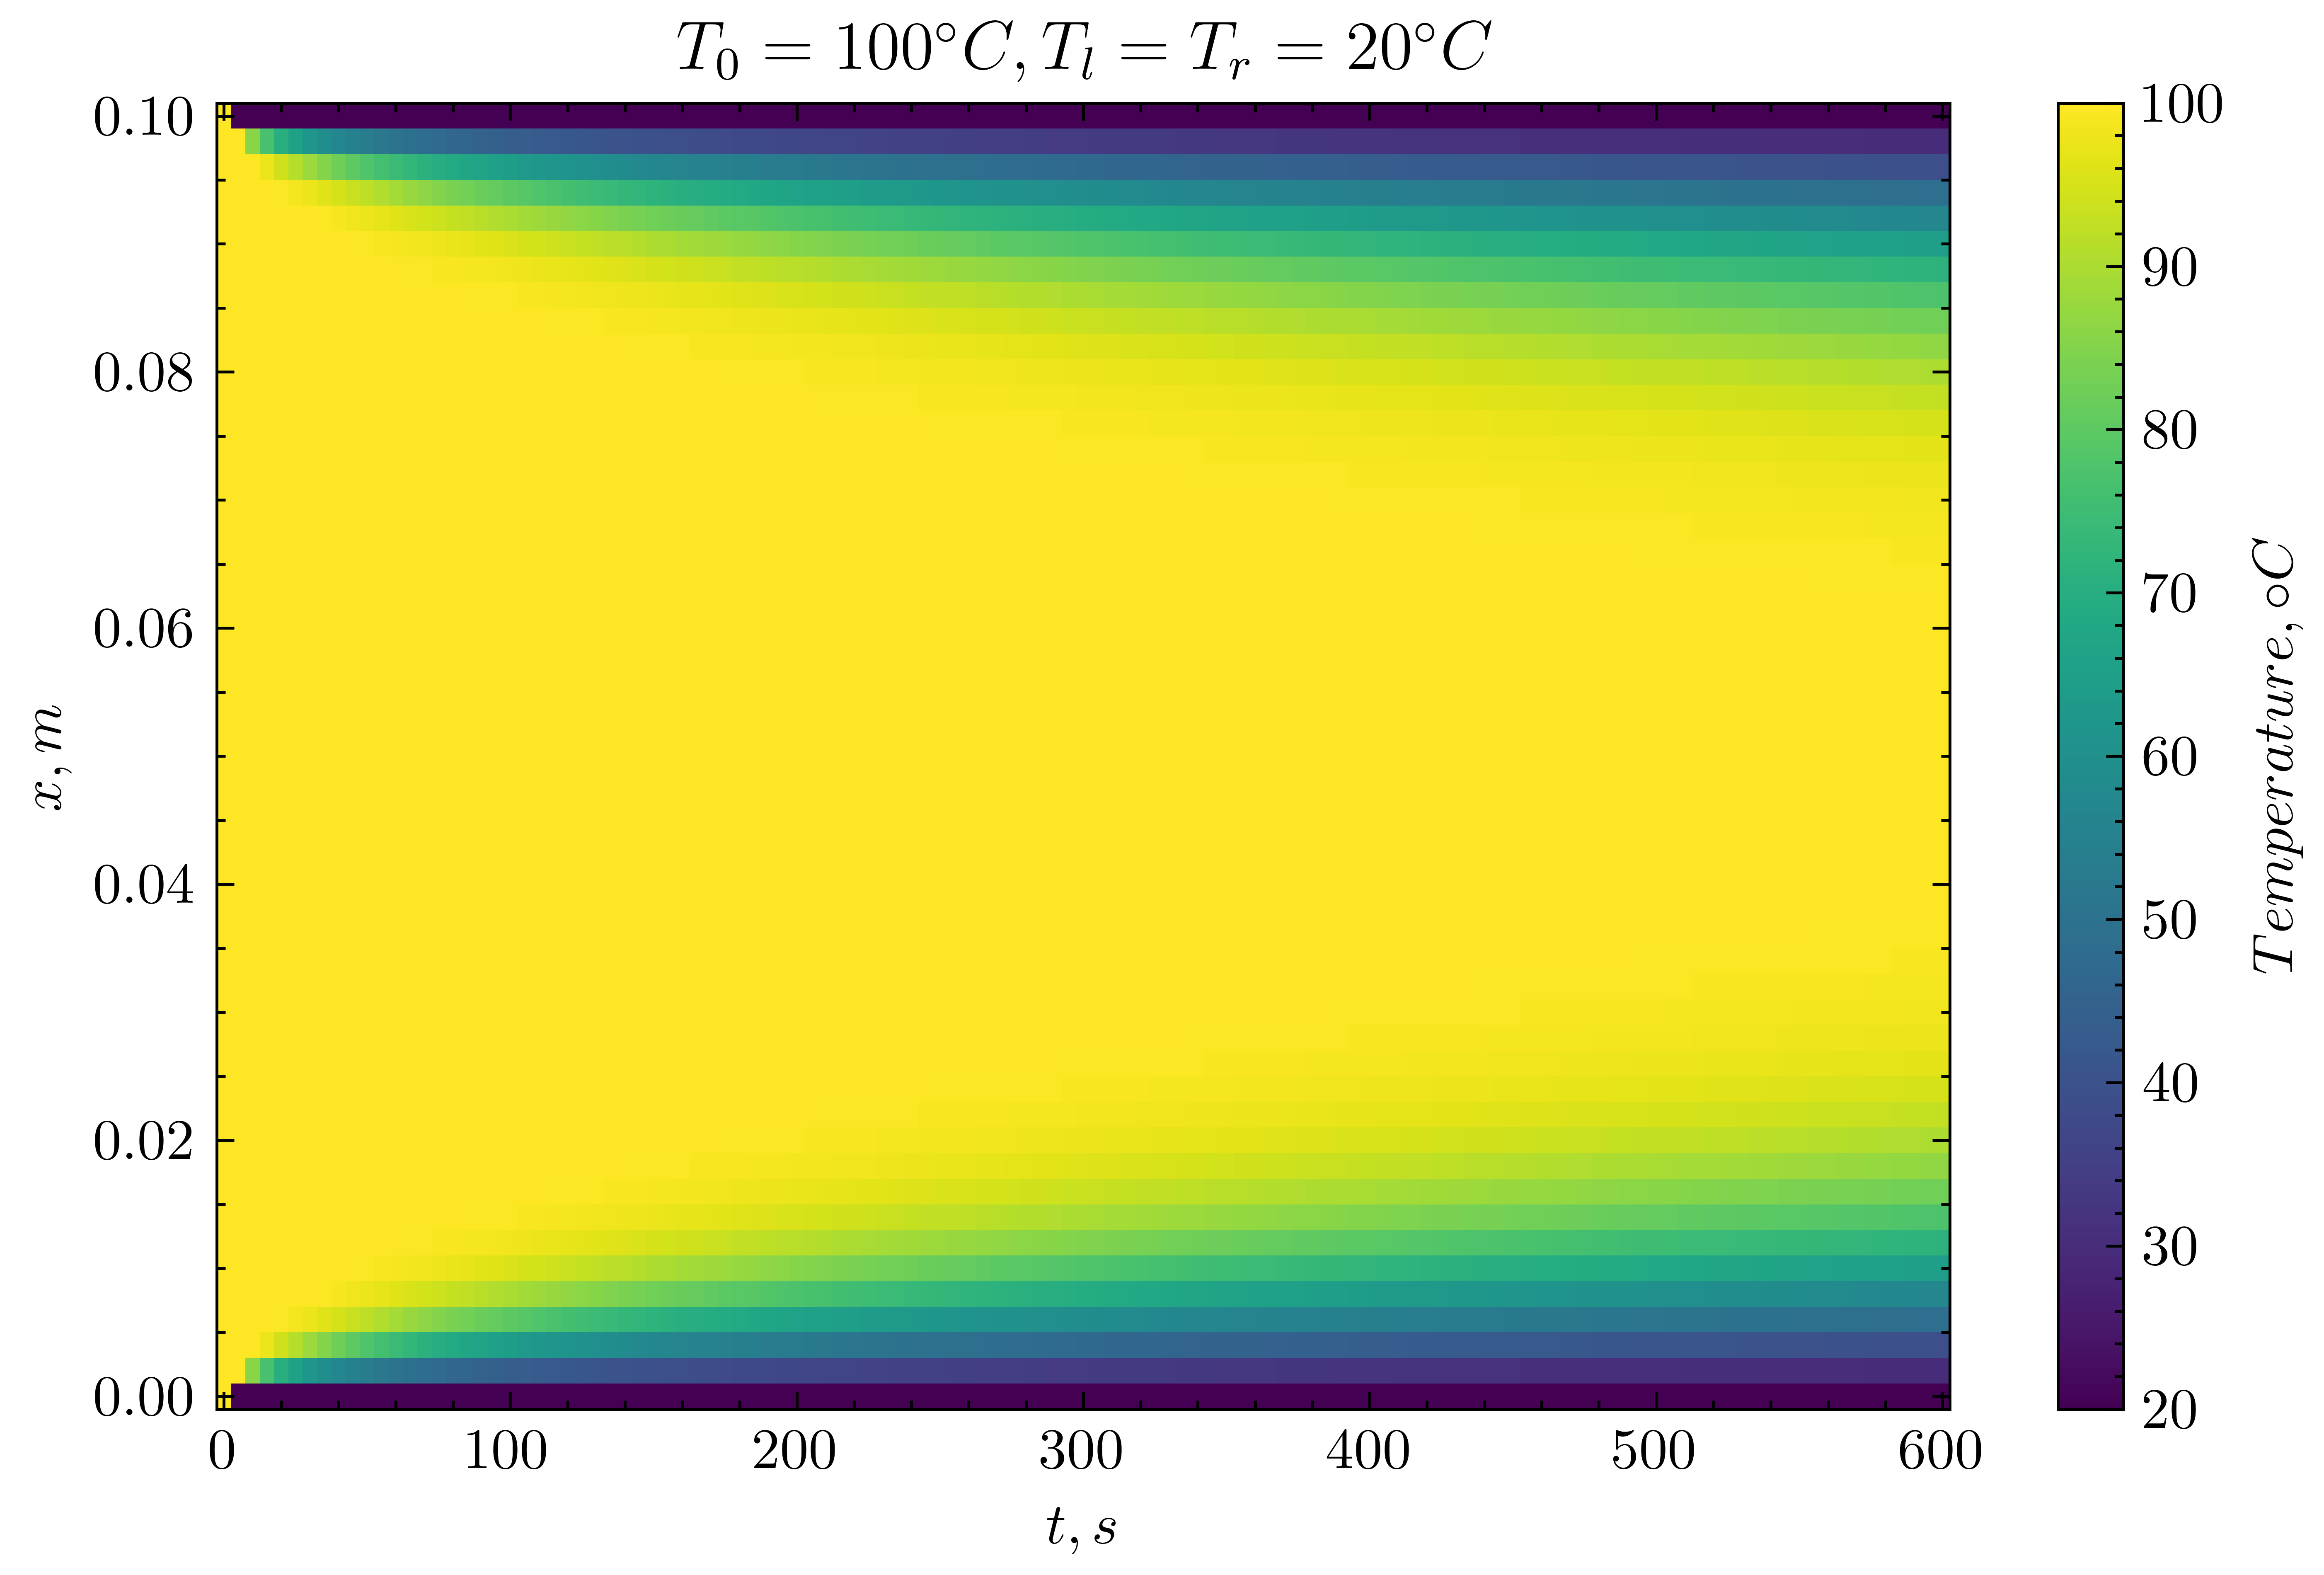
\includegraphics[]{2.1.png}
\end{center}
  \item Atrisināt siltumvadīšanas vienādojumu stienī, kur sākuma temperatūra ir $100^\circ C$, bet temperatūra uz viena stieņa gala ir $20^\circ C$, bet otrs gals ir izolēts. \\ Attēls problēmas atrisinājumam.
\begin{center}
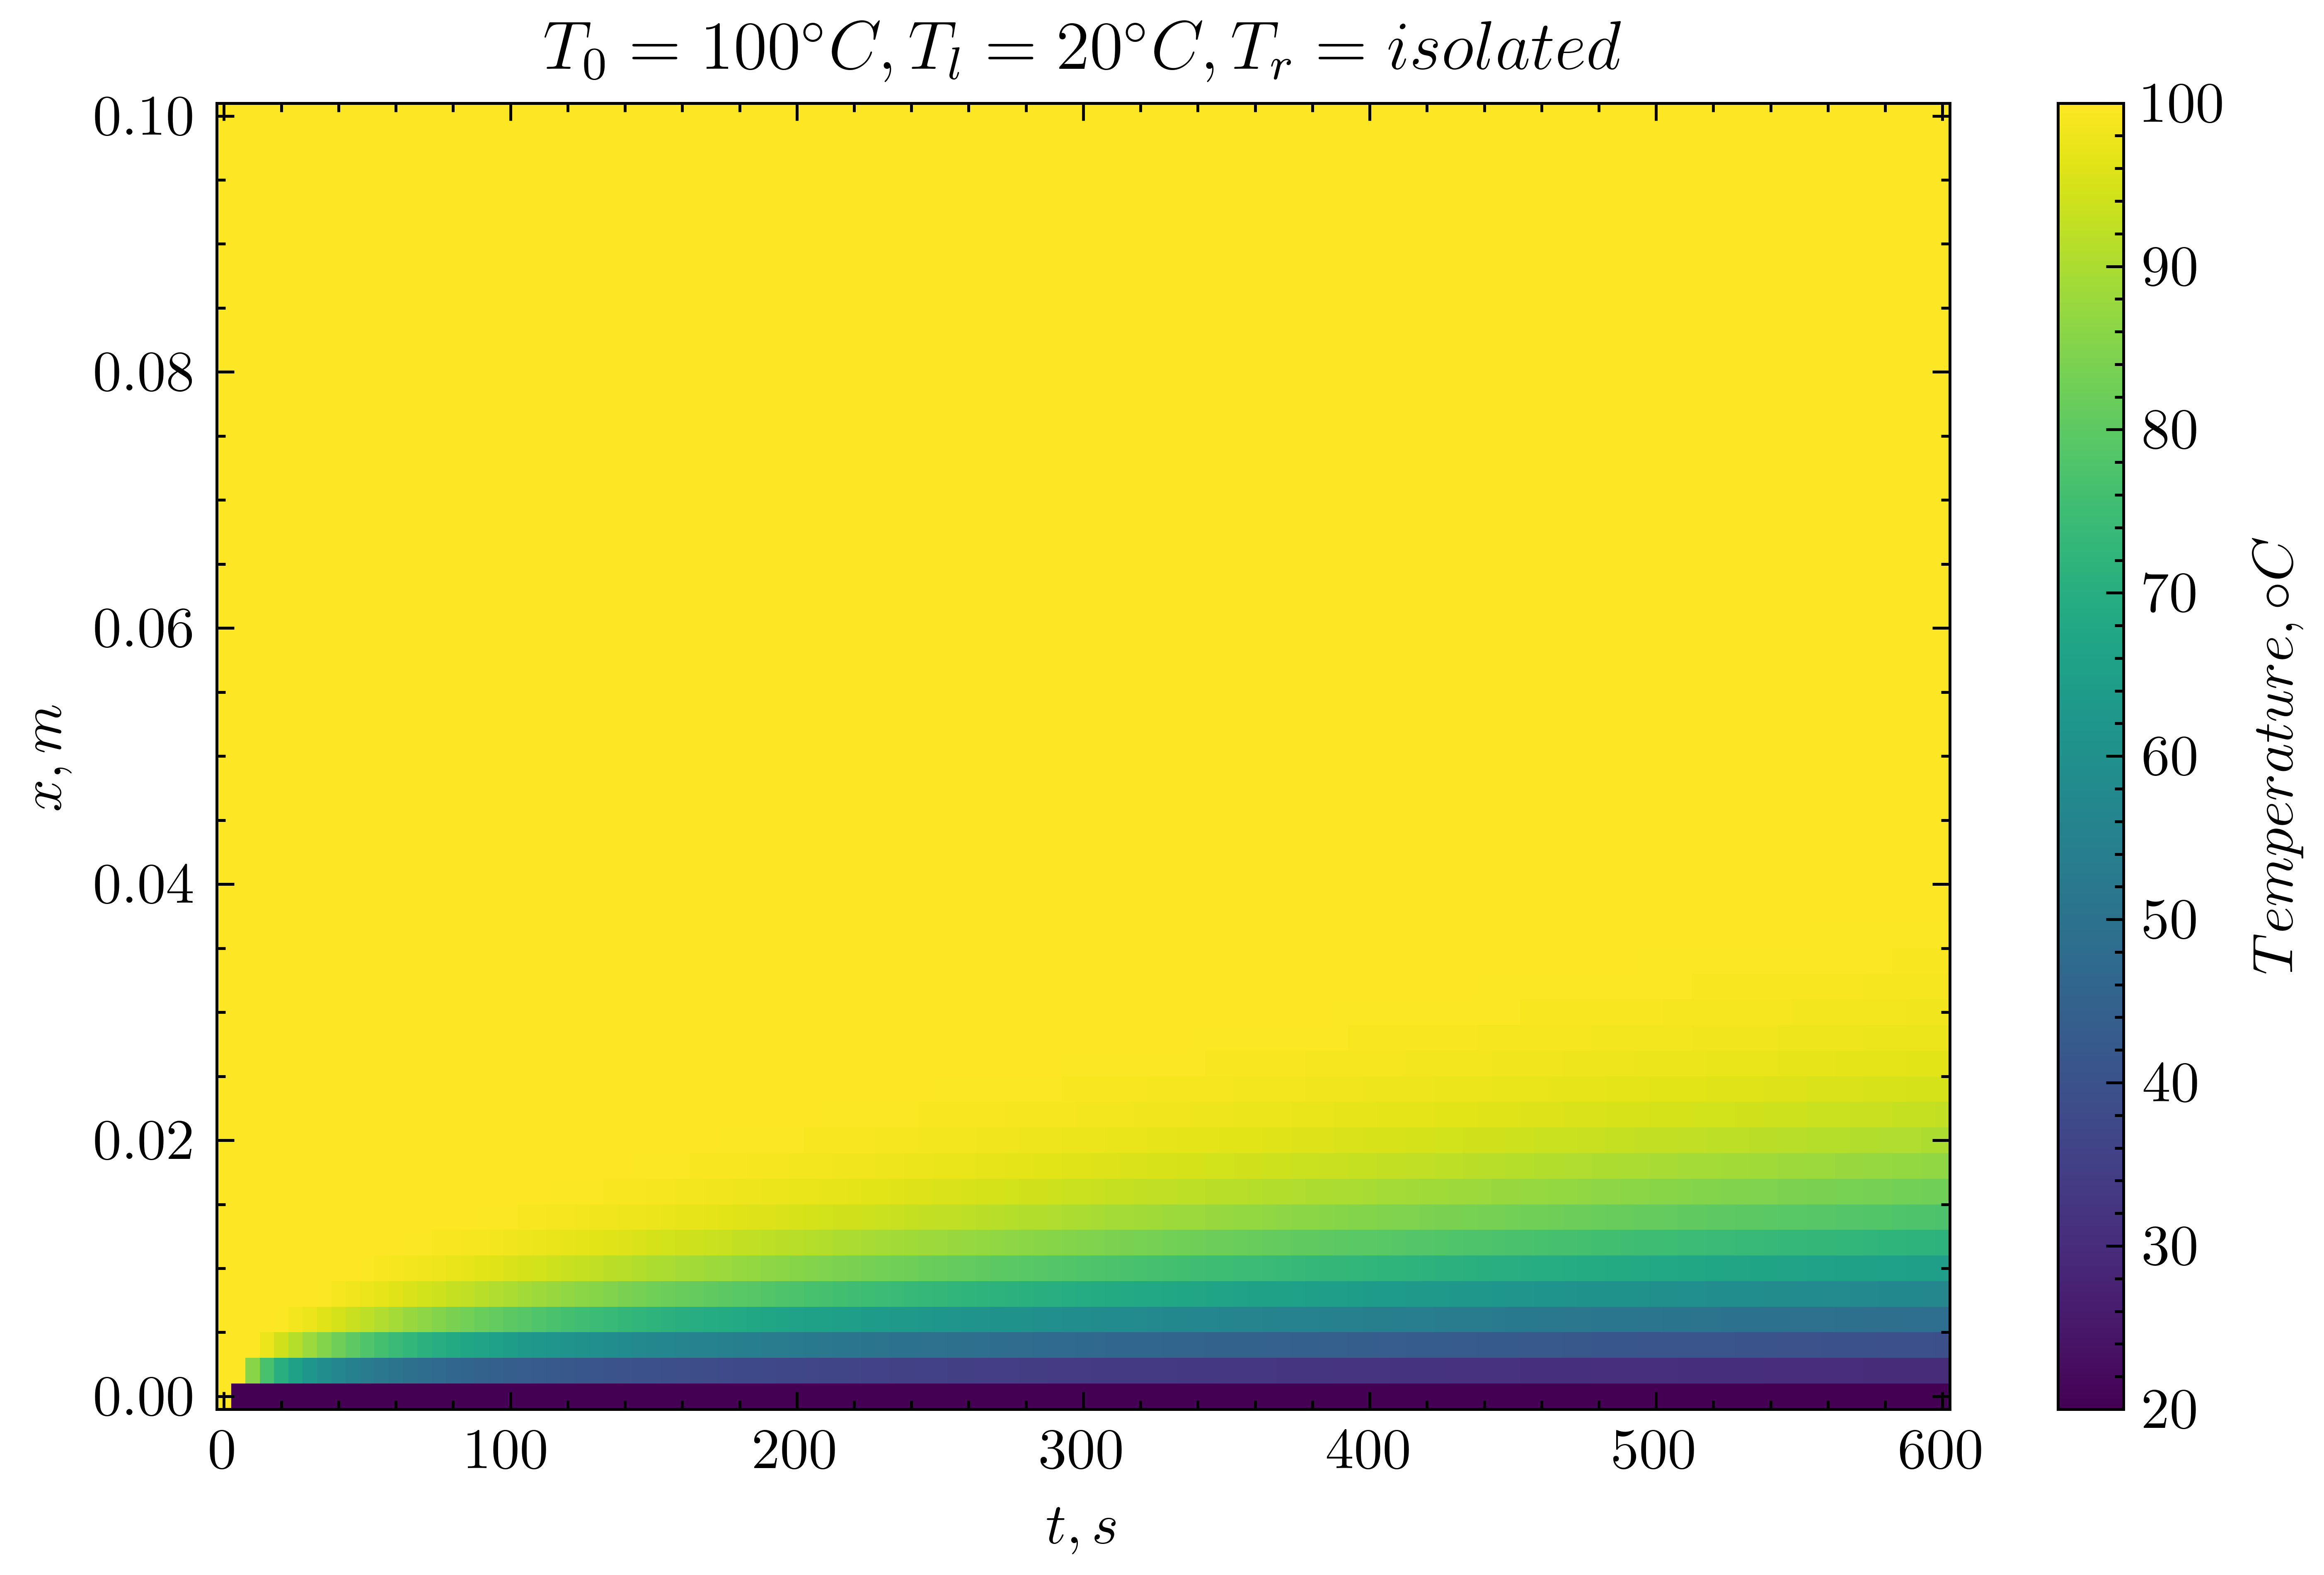
\includegraphics[]{2.2.png}
\end{center}
  \item Atrisināt siltumvadīšanas vienādojumu stienī, kur sākuma temperatūra ir $20\cdot \sin{\left(\frac{4\pi x}{l}\right)}$, bet abi stieņa gali ir izolēti. \\ Attēls problēmas atrisinājumam.
\begin{center}
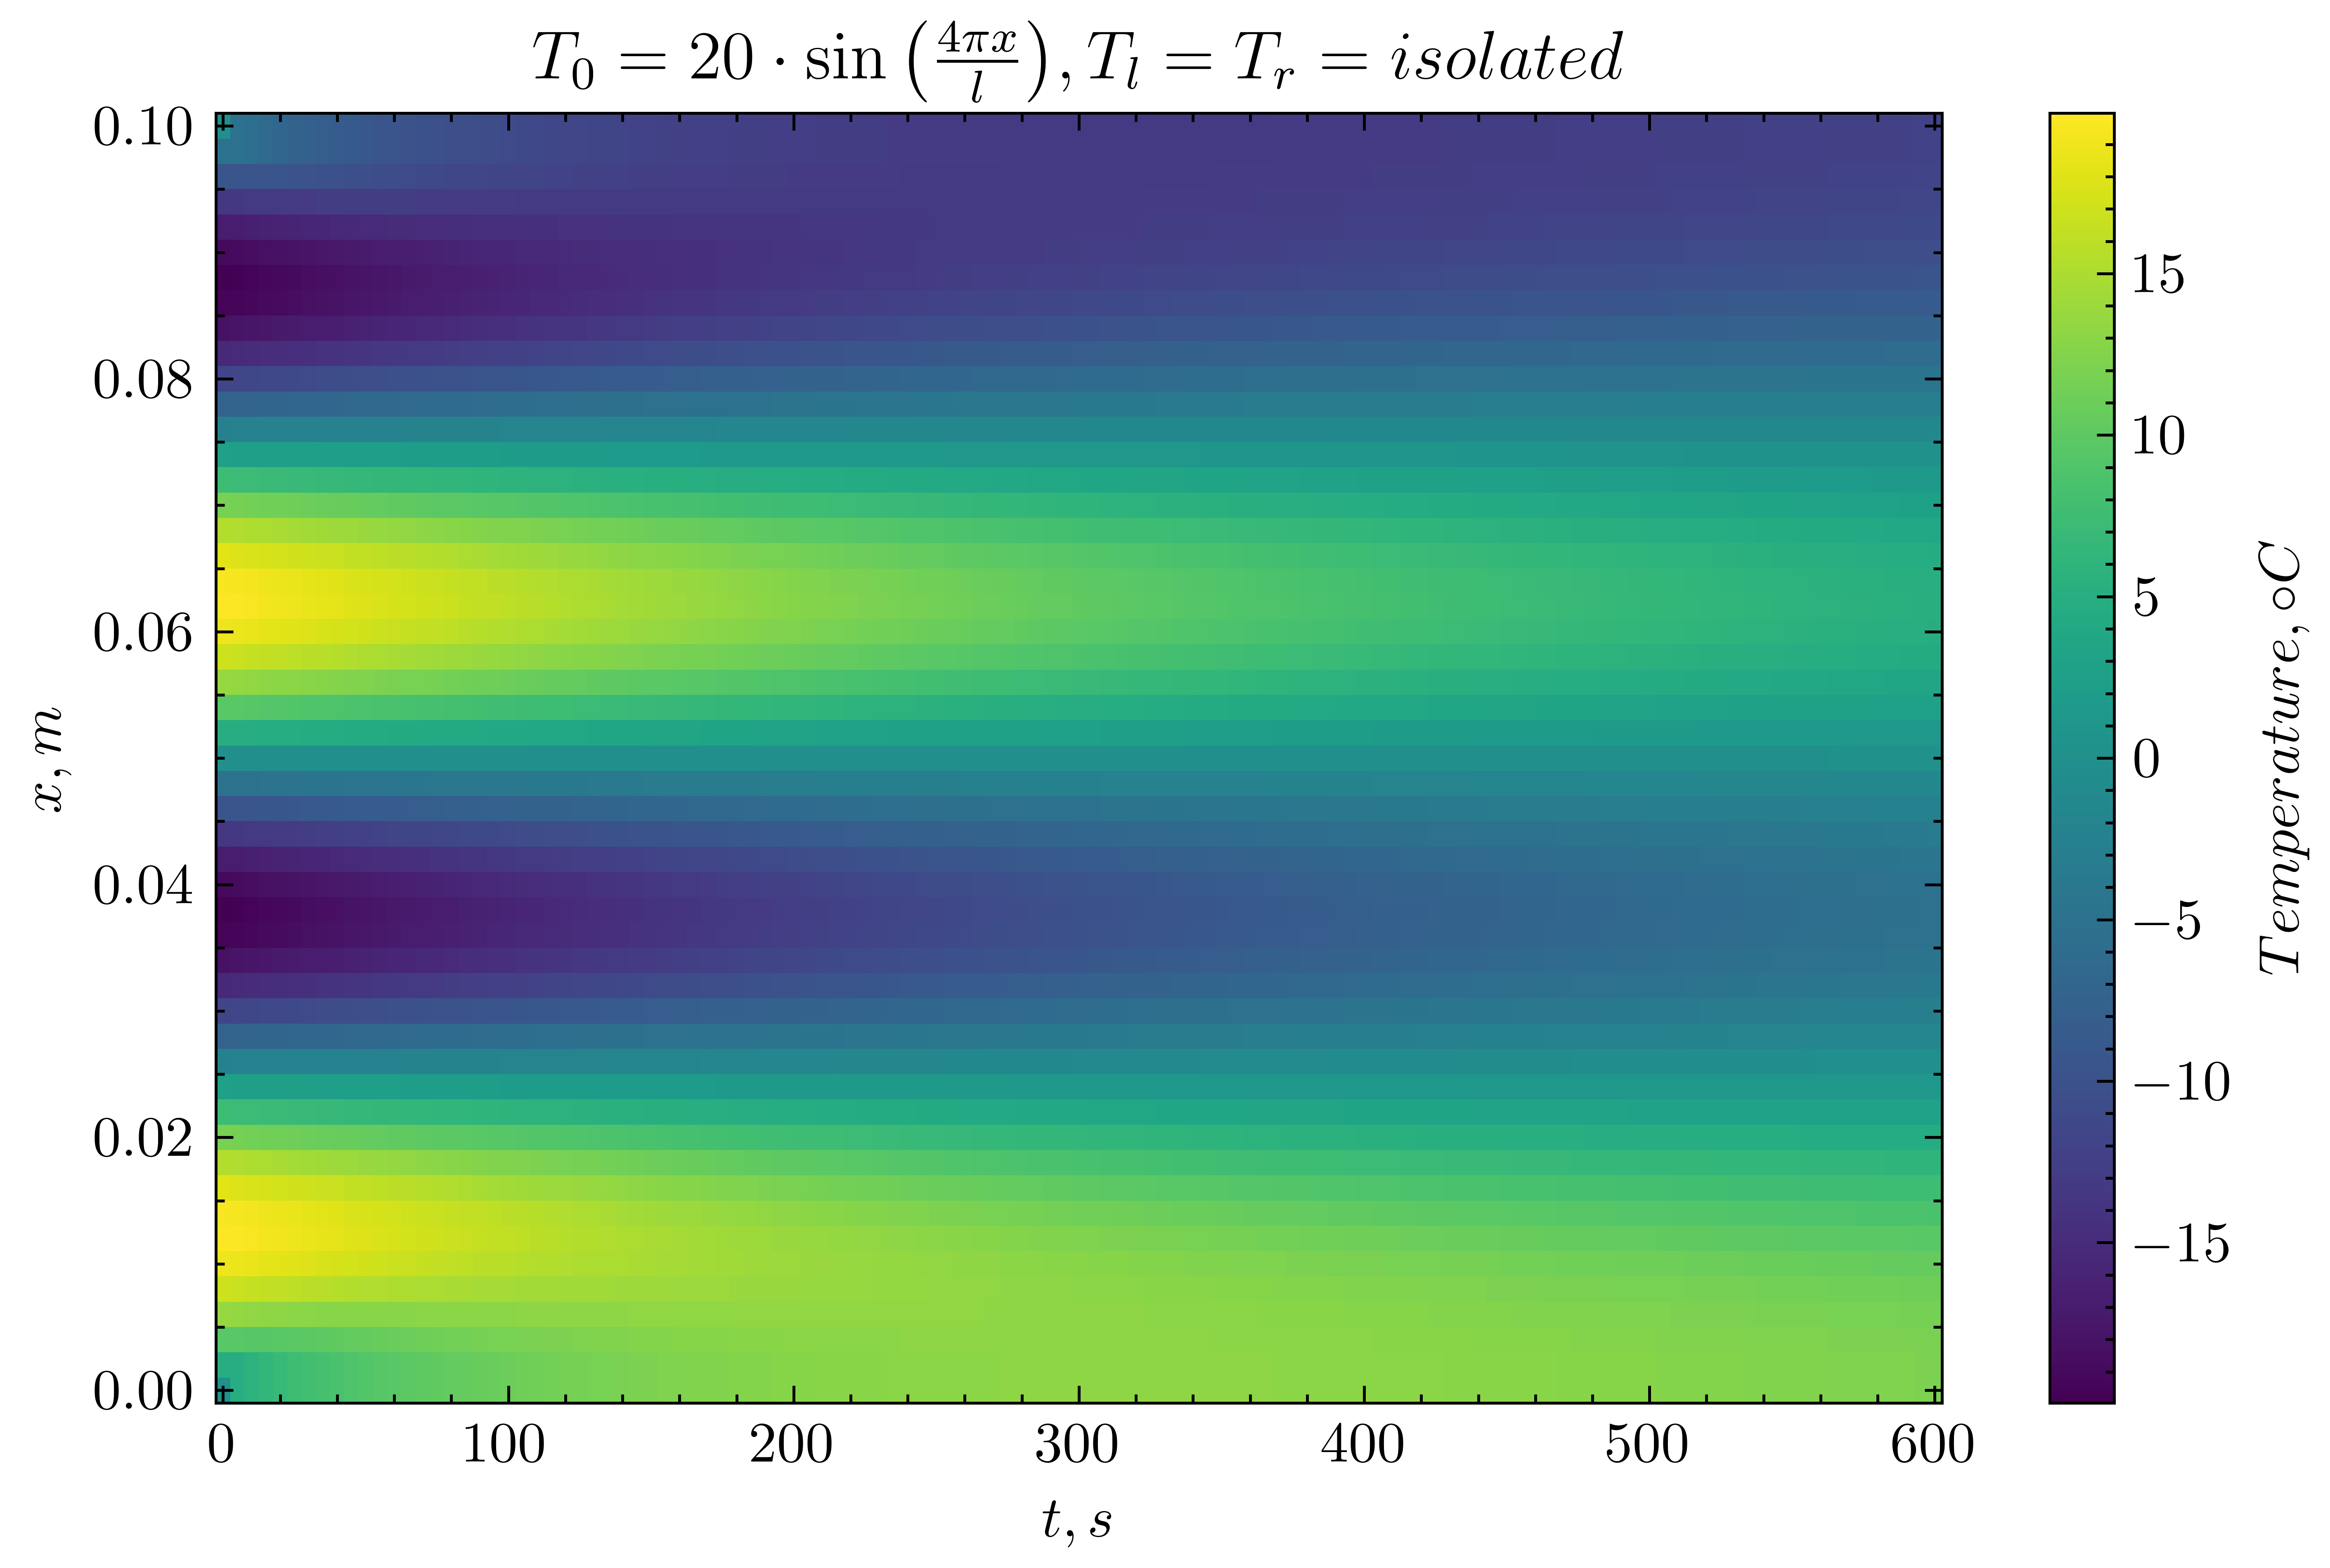
\includegraphics[]{2.3.png}
\end{center}
  \item Grafiks atrisinājumam ar skaitliskām nestabilitātēm.
\begin{center}
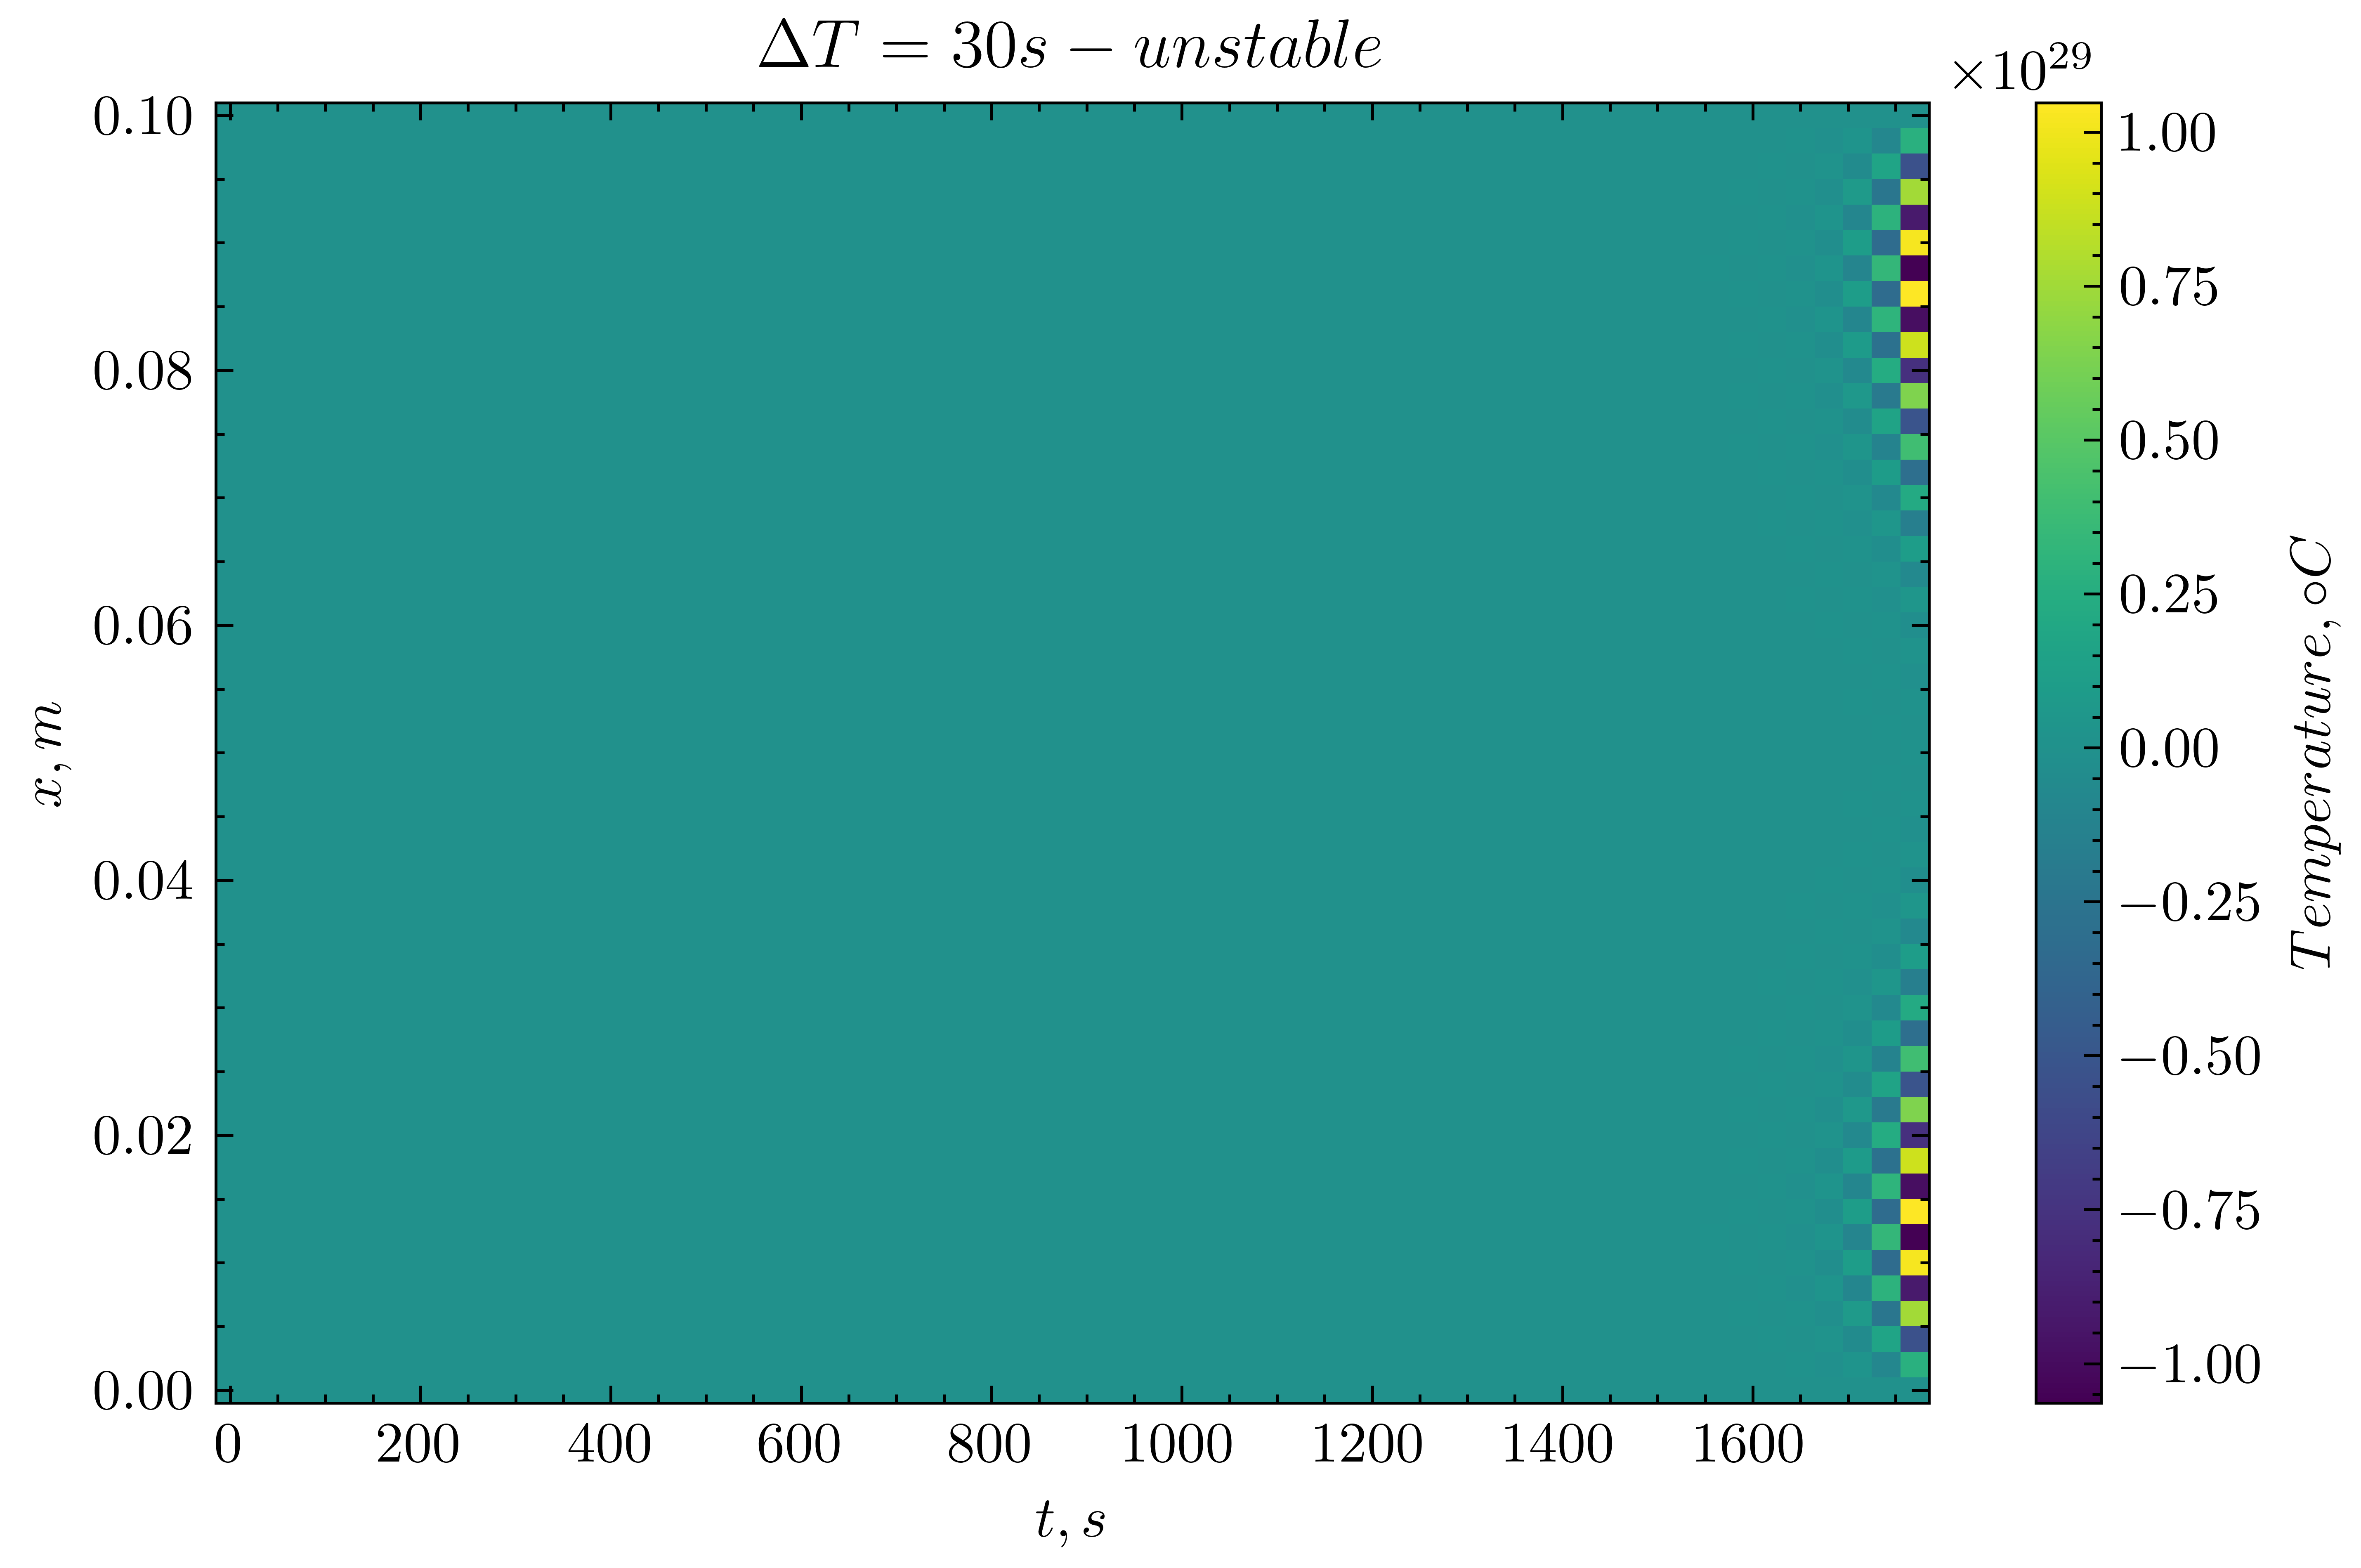
\includegraphics[]{2.4.png}
\end{center}
  \item \textbf{PAMATOJUMS:} Izmantotais kods siltumvadīšanas vienādojuma atrisināšanai.
  \begin{verbatim}
alpha = k / (rho * cp)
L = 0.10
N = 50
dx = L / N

# stability criterion for explicit FTCS: dt <= dx^2/(2*alpha)
dt_stable = 5.0
r = alpha * dt_stable / dx**2
(should be <= 0.5 for stability)

t_total = 600.0
simulated time (s)
steps = int(t_total / dt_stable) + 1
times = np.linspace(0, t_total, steps)

x = np.linspace(0, L, N + 1)

def lifeisasimulation(initial_T, bc_left, bc_right, dt, steps):
    """
    Simulate 1‑D heat conduction with explicit FTCS.
    bc_left, bc_right:
        - 'fixed': value (float) for Dirichlet
        - 'insulated': Neumann zero‑flux
    """
    T = initial_T.copy()
    T_record = np.empty((steps, N + 1))
    T_record[0] = T
    
    r_local = alpha * dt / dx**2
    
    for n in range(1, steps):
        T_new = T.copy()
        
        # interior points
        T_new[1:-1] = T[1:-1] + r_local * (T[2:] - 2.0 * T[1:-1] + T[:-2])
        
        # left boundary # lefty hehehe (:<
        if bc_left[0] == 'fixed':
            T_new[0] = bc_left[1]
        elif bc_left[0] == 'insulated':
            T_new[0] = T_new[1]    # ∂T/∂x = 0 → T0 = T1
        
        # right boundary # righty hahaha >:)
        if bc_right[0] == 'fixed':
            T_new[-1] = bc_right[1]
        elif bc_right[0] == 'insulated':
            T_new[-1] = T_new[-2]
        
        T = T_new
        T_record[n] = T
    
    return T_record

# 2nd point of the protocol
initial_T_case2 = np.full(N + 1, 100.0)
T_case2 = lifeisasimulation(initial_T_case2, ('fixed', 20.0),
('fixed', 20.0), dt_stable, steps)

# 3rd point of the protocol
initial_T_case3 = np.full(N + 1, 100.0)
T_case3 = lifeisasimulation(initial_T_case3, ('fixed', 20.0), 
('insulated', None), dt_stable, steps)

# my sanity is long gone, 4th point of the protocol
initial_T_case4 = 20.0 * np.sin(4 * np.pi * x / L)
T_case4 = lifeisasimulation(initial_T_case4, ('insulated', 
None), ('insulated', None), dt_stable, steps)

# what is blud waffling about, 6th point of the protocol
dt_unstable = 30.0
steps_unstable = 60
T_unstable = lifeisasimulation(initial_T_case2, ('fixed', 
20.0), ('fixed', 20.0), dt_unstable, steps_unstable)
  \end{verbatim}
\end{enumerate}

\newpage

\section*{Aprēķinu apakšprogrammas noformēšana}

\begin{enumerate}
    \item Izmantotais kods.
    \begin{verbatim}
class Heat1D:
"""
Explicit FTCS solver for 1-D heat-conduction equation.
Results returned as pandas.DataFrame (rows = time, columns = x).
"""
def __init__(self, L, N, dt, t_total, rho, cp, k):  # length, 
cells, time step, total time, density, coefficient, conductivity #
self.L, self.N = L, N
self.dx = L / N
self.dt = dt
self.t_total = t_total
self.steps = int(np.ceil(t_total / dt)) + 1

self.rho, self.cp, self.k = rho, cp, k
self.alpha = k / (rho * cp)
self.r = self.alpha * dt / self.dx**2

if self.r > 0.5:
    raise ValueError(f"Unstable: r = {self.r:.3f} > 0.5 "
                     "(reduce dt or refine grid)")

# coordinates and time vector
self.x = np.linspace(0.0, L, N + 1)
self.t = np.linspace(0.0, t_total, self.steps)

# placeholders for IC/BC (initial condition, boundary condition)
self.T0 = np.zeros_like(self.x)
self.bc_left = ('fixed', 0.0)      # default Dirichlet 0 °C
self.bc_right = ('fixed', 0.0)

# ---------- setters -------------------------------------------------
def set_initial(self, T0):
"""T0: scalar, 1-D array of size N+1, or callable f(x)."""
if np.isscalar(T0):
    self.T0[:] = T0
elif callable(T0):
    self.T0[:] = T0(self.x)
else:
    T0 = np.asarray(T0, dtype=float)
    if T0.shape != self.x.shape:
        raise ValueError("T0 length must be N+1")
    self.T0[:] = T0

def set_boundary(self, left, right):
"""
left, right : tuple ('fixed', value) or ('insulated', None)
"""
self.bc_left = left
self.bc_right = right

# ---------- core solver ---------------------------------------------
def solve(self):
T = self.T0.copy()
out = np.empty((self.steps, self.N + 1), dtype=float)
out[0] = T

for n in range(1, self.steps):
    T_new = T.copy()
    # interior nodes
    T_new[1:-1] = (T[1:-1] +
                   self.r * (T[2:] - 2.0*T[1:-1] + T[:-2]))

    # left BC
    if self.bc_left[0] == 'fixed':
        T_new[0] = self.bc_left[1]
    elif self.bc_left[0] == 'insulated':
        T_new[0] = T_new[1]

    # right BC
    if self.bc_right[0] == 'fixed':
        T_new[-1] = self.bc_right[1]
    elif self.bc_right[0] == 'insulated':
        T_new[-1] = T_new[-2]

    T = T_new
    out[n] = T

# build DataFrame: index=time, columns=x coordinate
df = pd.DataFrame(out, index=self.t, columns=self.x)
df.index.name = "time_s"
df.columns.name = "x_m"
return df
    \end{verbatim}
\end{enumerate}

\newpage
\renewcommand{\refname}{Izmantotā literatūra}
\nocite{*}
\bibliographystyle{plain}
\bibliography{bibliography}
\end{document}